\documentclass[conference]{IEEEtran}
\IEEEoverridecommandlockouts
% The preceding line is only needed to identify funding in the first footnote. If that is unneeded, please comment it out.
\usepackage{cite}
\usepackage{amsmath,amssymb,amsfonts}
\usepackage{algorithmic}
\usepackage{graphicx}
\usepackage{textcomp}
\usepackage{xcolor}
\usepackage{array}

\newcommand*{\vertbar}{\rule[-1ex]{0.5pt}{2.5ex}}

\def\BibTeX{{\rm B\kern-.05em{\sc i\kern-.025em b}\kern-.08em
    T\kern-.1667em\lower.7ex\hbox{E}\kern-.125emX}}
\begin{document}

\title{Mechanical field reconstruction from limited observations
\\
{\footnotesize \textsuperscript{*}Note: Sub-titles are not captured in Xplore and
should not be used}
\thanks{Identify applicable funding agency here. If none, delete this.}
}

\author{\IEEEauthorblockN{ Bahador Bahamani}
\IEEEauthorblockA{\textit{CEEM Department} \\
\textit{Columbia University}\\
NY, USA\\
bb2969@columbia.edu}
}

\maketitle

\begin{abstract}
In this project, we aim to reconstruct temperature field (as a case study) from a few noisy measurements which is similar to the real experimental conditions. To this end, we propose a dictionary learning approach that tries to find a sparse combination of dictionary elements. We find such sparse weights using basis pursuit and LASSO formalism and compare these optimization formulations. In this work, the dictionary is constructed with a priori reliable solutions, e.g., from numerical solvers, without any transformation.
\end{abstract}

\begin{IEEEkeywords}
component, formatting, style, styling, insert
\end{IEEEkeywords}

\section{Introduction}
In mechanical engineering, we have inevitable limitations regarding the number and location of sensors for an experimental task. These limitation could be related to expensiveness of  sensors or manufacturing restrictions about accessibility of different locations on the surface of samples or inside the samples. On the other hand, we are interested to have as much as possible more information about the entire body of sample to conduct analysis more rigorously. Another concern is that experimental observations come with unavoidable level of noise. Thus, it would be very helpful if we could find a robust approach that can reconstruct a full field from limited and noisy measurements. Due to amazing successes in the field of sparse modeling, we are interested to try some of those ideas in the field of mechanics and specially for heat transfer experiments of heterogeneous materials, in this project. Although we have tried heat transfer problem, the approach could be used for other applications such as stress analysis.

The idea of using sparse modeling to reconstruct a mechanical field is first introduced by \cite{CallahamRobust2019} for fluid dynamics applications. The main idea of their approach comes from the seminal work of \cite{WrightRobust2008} where they introduce a robust approach for image recognition using sparse representation and dictionary learning. In another line of research, \cite{Erichson2020} introduces a neural network based method for field reconstruction from limited measurements, again for fluid dynamics applications. Our method used in this manuscript is similar to \cite{CallahamRobust2019,WrightRobust2008} but for a different domain application.

In this project, we assume that governing equations of the heat transfer experiment are completely known to use and the actual experimental data should satisfy the conservation of energy if the experiment is conducted perfectly fine without noise. Therefore, we hypothesize that if sufficiently many admissible solutions (e.g., from a numerical simulator) are collected with the same boundary condition as the actual experiment, then the experimental observation can be represented as a linear combination of those admissible solutions.

\section{Technical Approach}
For a state vector $y \in \mathbb{R}^n$ which represents a mechanical field, for example temperature, over a set of grid points, we are interested to find and its approximation called $y^h \in \mathbb{R}^n$ by knowing a subset of its components $y_{\text{meas}} = M y$ where $y_{\text{meas}} \in \mathbb{R}^m$ and $m<<n$. We assume that $y$ admits a linear combination of library elements $\{ \psi_j \} \in \mathbb{R}^n$ where $j=1,2,\dots,r$, hence we have:
\begin{equation}
y^h \approx \mathbf{\Psi} c = 
\begin{pmatrix}
\mid & \mid & & \mid \\
\psi_1 & \psi_2 & \cdots & \psi_r\\
\mid & \mid & & \mid \\
\end{pmatrix}
c,
\end{equation}
where $c \in \mathbb{R}^r$ is the coefficient vector that indicates the contribution of each mode presented in the library $\mathbf{\Psi} \in \mathbb{R}^{n\times r}$. Within this set-up, the reconstruction problem is equivalent to finding an appropriate coefficient vector that can satisfy the following condition:
\begin{equation}
y_{\text{meas}}^h \approx M\mathbf{\Psi}\hat{c},
\end{equation}
where $\hat{c}$ is an unknown coeficient vector that must be found such that the right hand side in the above equation be as much as close to the left hand side according to an appropriate metric (e.g., L2-norm). As mentioned, in real application the number of measurements are much less than the total degrees of freedom in the underlying mechanical system, and hence the above equation is underdetermined ($m<r$). It is well-accepted that most of the physical problems admit a form of sparse representation (at least from empirical perspective) in the ambient space or an appropriate transformed space such as Fourier or wavelet space. Therefore, it is natural to assume the coefficient vector has sparsity structure to regularize the above mentioned problem.

To promote sparsity in the coefficient vector, we can reformulate the problem with different optimization formulations. Here, we consider two approaches: 1-basis pursuit regression and 2-LASSO regression. In the context of basis pursuit, we look for the sparsest coefficient $\hat{c}$ in the L1-norm sense such that:
\begin{equation}
\hat{c} = \underset{c}{\text{argmin}} ||c||_1 \ \text{s.t.} \ y_{\text{meas}} = M\mathbf{\Psi}\hat{c}, 
\end{equation}
when there is no noise in the data. For noisy measurements we have:
\begin{equation}
\hat{c} = \underset{c}{\text{argmin}} ||c||_1 \ \text{s.t.} \ ||y_{\text{meas}}-M\mathbf{\Psi}\hat{c}||_2 < \epsilon, 
\end{equation}
where $\epsilon$ is an hyperparametr that controls the level of deviation of the reconstructed measurements from noisy measurements. In the LASSO regression we solve the following optimization problem for regardless having noisy data or not:
\begin{equation}
\hat{c} = \underset{c}{\text{argmin}}  ||y_{\text{meas}}-M\mathbf{\Psi}\hat{c}||_2 + \lambda ||c||_1,
\end{equation}
where $\lambda$ is a penalty parameter that controls the level of sparsity in the coefficient vector. In this project, we formulate these convex optimization problem using \texttt{cvxpy} package \cite{Diamond2016}.

\section{Data generation and process}
As mentioned earlier, our approach relies on a dictionary consist of sufficiently many admissible solutions that satisfy the underlying governing equations of heat transfer with boundary and initial conditions similar to the actual. Therefore, we need to collect such solutions as elements of our library.  We assume heat conduction is the only heat transfer mechanism in the actual experiment, hence the conservation of energy leads to the following parabolic partial differential equation (PDE):
\begin{equation}
\rho c_T \frac{\partial T}{\partial t} - \nabla . (-\kappa(x,t) \nabla T(x,t)) =0,
\end{equation}
where $\rho$, $c_T$, $T(x,t)$, $\kappa(x,t)$, $x$, and $t$ are density, heat capacity, temperature field, heat conductivity, spatial coordinate and time, respectively. In this project, we use euler method to discretize the above PDE in time and utilize Galerkin approximation to discretize in space within the context of finite element method (FEM). We have implemented our simulator in an open-source FEM library called \texttt{fenics} \cite{Alnaes2015}.

Typically our mesh for use in FEM has a an irregular topology (see Fig. \ref{fig::mesh}) and does not look like an square shaped grid which is common for sensor placement in an experimental test or images in computer vision studies. To be as much as close to the experiential conditions, we perform some basic image processing operations including (1) binarizing temperature field as a single color in gray scale, (2) cropping image to exclude the boundary effects, and (3) down sampling the image to reduce the computational cost for later optimization tasks. These basic image processing operations are performed with an open-source packaeg called \texttt{scikit-image} \cite{Walt2014}. Figure \ref{fig::img-proc} shows two snapshots before and after this process.

\begin{figure}[!ht]
  \centering
  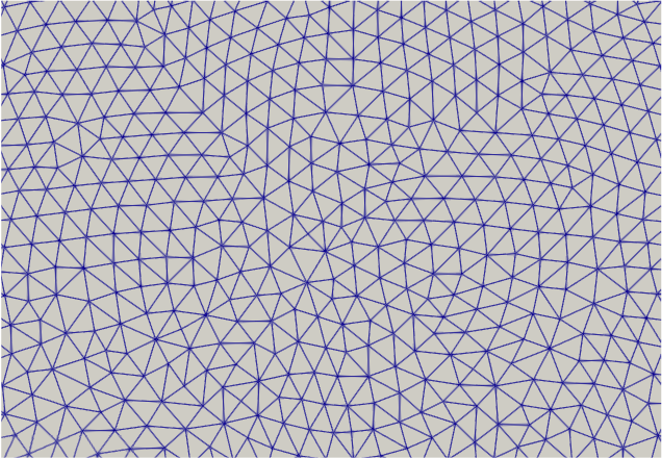
\includegraphics[width=0.3\textwidth]{figure/mesh.png}
  \caption{a zoomed window of the used FEM mesh.}\label{fig::mesh}
\end{figure}

\begin{figure}[!ht]
  \centering
  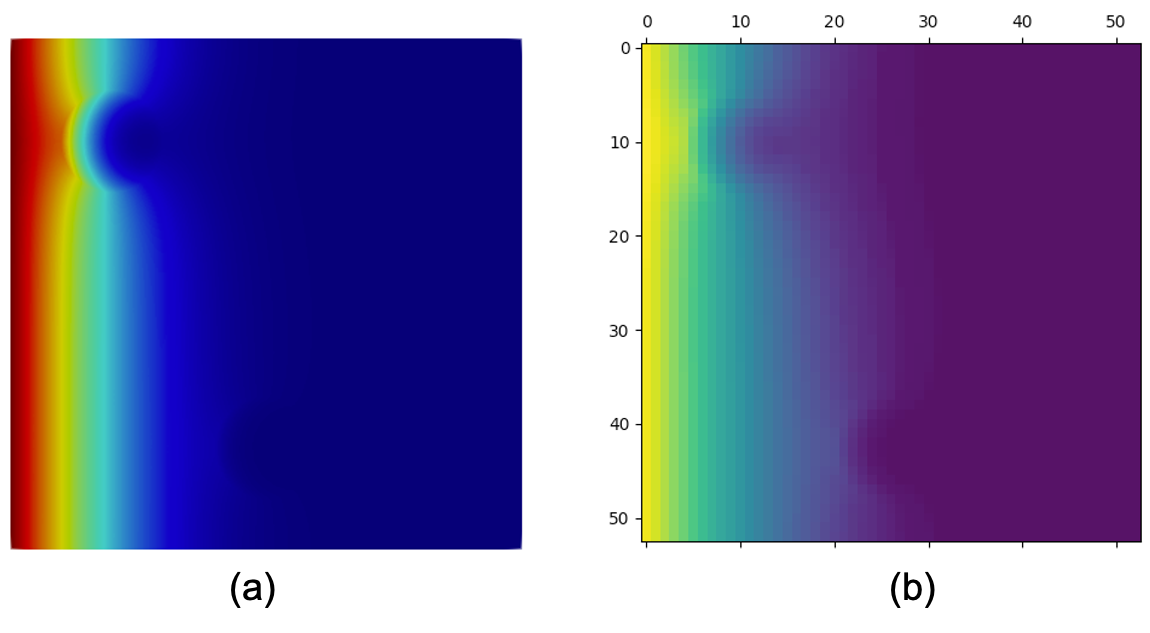
\includegraphics[width=0.4\textwidth]{figure/image_proc.png}
  \caption{(a) high resolution image from nodal solution of FEM shown in \texttt{paraview} software \cite{Ahrens2005} and (b) binarized an down sampled image ($55\times55$ pixels) for use in the optimization task. Notice that these images are not corresponding to each other; we just show two cases as illustration.}\label{fig::img-proc}
\end{figure}

\section{Experiments}
In this section, we first introduce a toy example which doesn't require any numerical simulator to construct the library. This allows interested reader tries the main idea with a simpler problem at hand, and also it is a good practice for verification exercise. In the second example, we solve our target heat transfer problem.

\subsection{artificial data with known analytical expression}
We generate a 1000 snapshots of a target field at different times $t \in [0, 10]$ with the following expression:
\begin{equation}
y = c_1 \exp(-\frac{(x-x_1)^2}{2\sigma_1^2}) \sin(2\pi f_1 t)+
    c_2 \exp(-\frac{(x-x_2)^2}{2\sigma_2^2}) \sin(2\pi f_2 t).
\end{equation}
The parameters we used for data generation are $c_1=1$, $x_1=0.5$, $\sigma_1=0.6$, $f_1=1.3$, $c_2=1.2$, $x_2=-0.5$, $\sigma_2=0.3$, and $f_2=4.1$. We regularly sample spatial coordinate $x \in [-2, 2]$ with 400 points. 300 snapshots are randomly selected to built our dictionary and, measurements are gathered from 8 random points among the 400 possible places on the $x$ axis. Therefore, in this problem we have $n=400$, $r=300$, and $m=8$. Note that we normalize our data along the temporal axis to have zero mean and unit standard deviation.


\bibliography{mybibfile}

\begin{thebibliography}{00}
\bibitem{CallahamRobust2019} Callaham, Jared L., Kazuki Maeda, and Steven L. Brunton. ''Robust flow reconstruction from limited measurements via sparse representation.'' Physical Review Fluids 4.10 (2019): 103907.
%
\bibitem{WrightRobust2008} Wright, John, et al. "Robust face recognition via sparse representation." IEEE transactions on pattern analysis and machine intelligence 31.2 (2008): 210-227.
%
\bibitem{Erichson2020} Erichson, N. Benjamin, et al. "Shallow neural networks for fluid flow reconstruction with limited sensors." Proceedings of the Royal Society A 476.2238 (2020): 20200097.
%
\bibitem{Diamond2016} Diamond, Steven, and Stephen Boyd. "CVXPY: A Python-embedded modeling language for convex optimization." The Journal of Machine Learning Research 17.1 (2016): 2909-2913.
%
\bibitem{Alnaes2015} Alnaes, Martin, et al. "The FEniCS project version 1.5." Archive of Numerical Software 3.100 (2015).
%
\bibitem{Walt2014} Van der Walt, Stefan, et al. "scikit-image: image processing in Python." PeerJ 2 (2014): e453.
%
\bibitem{Ahrens2005} Ahrens, James, Geveci, Berk, Law, Charles, ParaView: An End-User Tool for Large Data Visualization, Visualization Handbook, Elsevier, 2005, ISBN-13: 978-0123875822
%
\end{thebibliography}

\vspace{12pt}


\end{document}
